\section{Level 1 Pipelines}
\label{sec:ap}

\begin{figure}[th]
\begin{center}
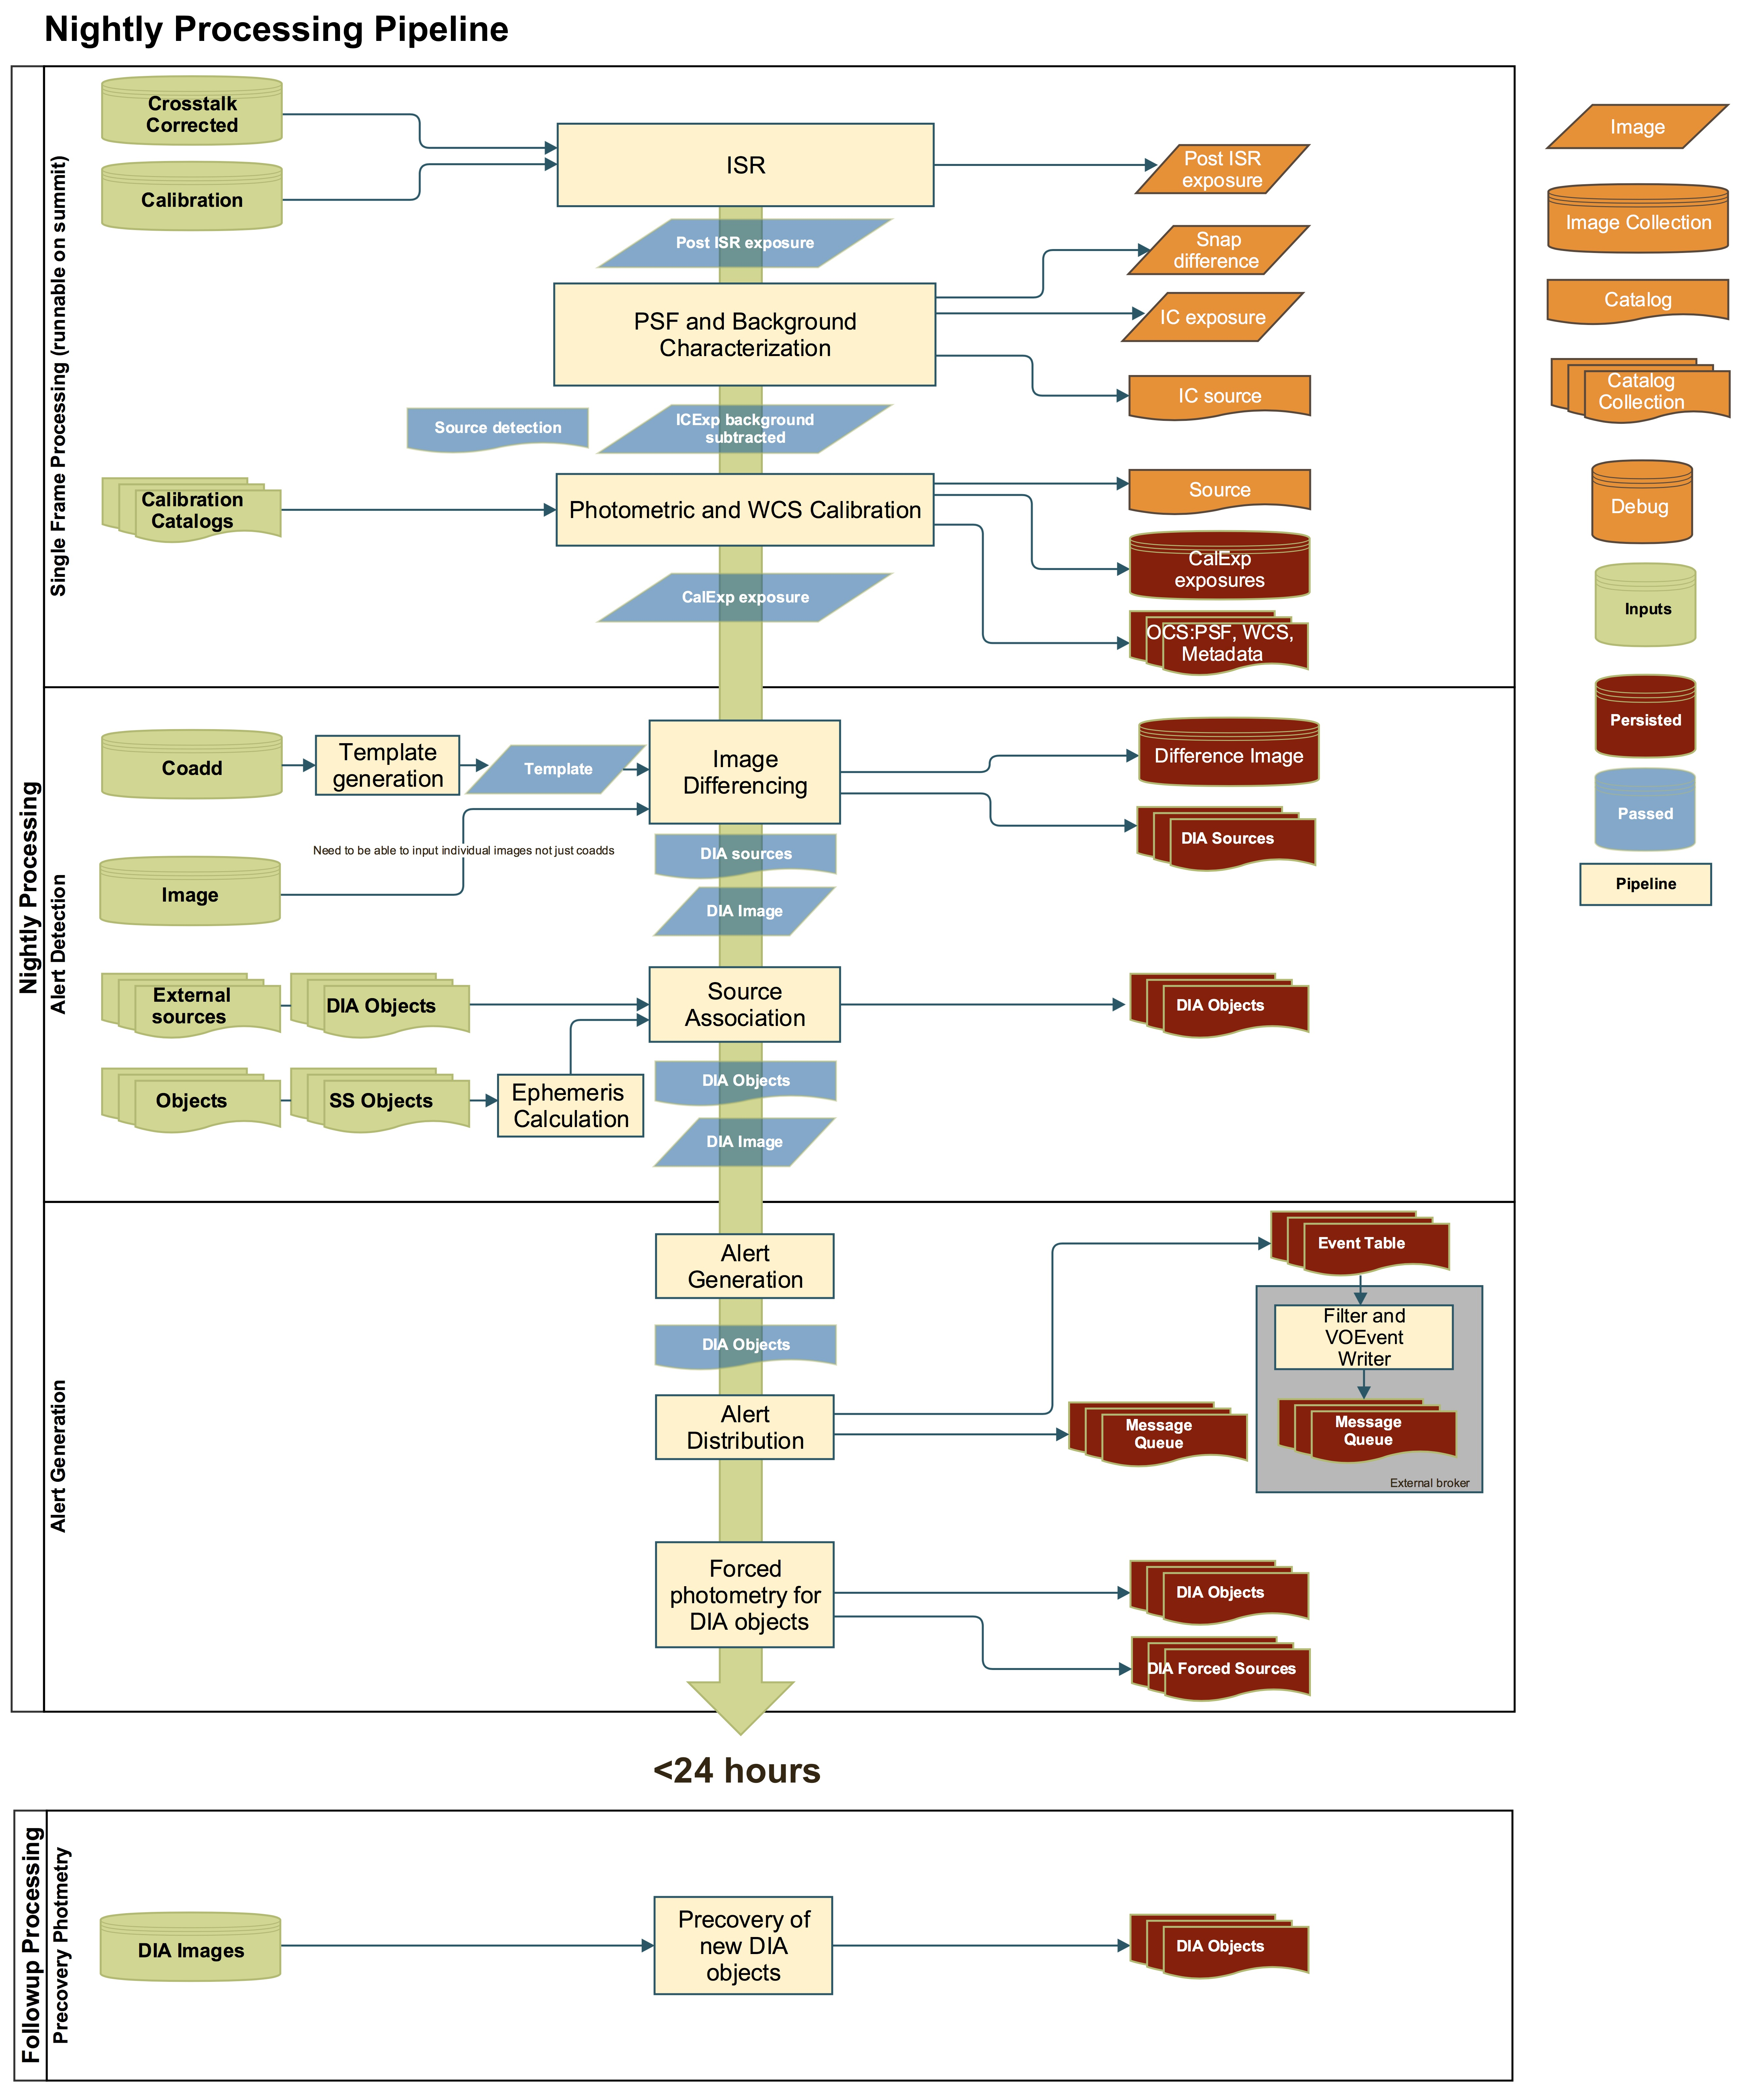
\includegraphics[width=0.9\textwidth]{figures/Level_1_Processing_Flowchart.jpg}
\caption{\label{fig:nightly} The nightly processing flowchart
  describing the flow of images and data through single frame
  processing, image differencing, alert generation and production}
\end{center}
\end{figure}

\subsection{Single Frame Processing Pipeline (\wbsSFM)}
\label{sec:apSingleFrameProcessing}

\subsubsection{Key Requirements}

Single Frame Processing (SFM) Pipeline is responsible for reducing raw image data to \emph{calibrated exposures}, and detection and measurement of \Sources (using the components functionally a part of the Object Characterization Pipeline).
\\

SFM pipeline functions include:
%
\begin{itemize}
    \item Assembly of per-amplifier images to an image of the entire CCD;
    \item Instrumental Signature Removal;
    \item Cosmic ray rejection and snap combining;
    \item Per-CCD determination of zeropoint and aperture corrections;
    \item Per-CCD PSF determination;
    \item Per-CCD WCS determination and astrometric registration of images;
    \item Per-CCD sky background determination;
    \item Source detection and measurement
\end{itemize}

Calibrated exposure produced by the SFM pipeline must possess all information necessary for measurement of source properties by single-epoch Object Characterization algorithms.

It shall be possible to run this pipeline in two modes: a ``fast" mode needed in nightly operations for Level 1 data reductions where no source characterization is done beyond what's required for zero-point, PSF, sky, and WCS determination (image reduction); and a ``full" mode that will be run for Level 2 data reductions.

\subsubsection{Baseline Design}

Single Frame Processing pipeline will be implemented as a flexible framework where different data can be easily treated differently, and new processing steps can be added without modifying the stack code.
\\

It will consist of three primary components:
%
\begin{itemize}
    \item A library of useful methods that wrap a small number of atomic operations (e.g., {\tt interpolateFromMask}, {\tt overscanCorrection}, {\tt biasCorrection}, etc.) % RHL things like overscanCorrection aren't atomic (or at least, they use afw::math and afw::cameraGeom primitives)
    \item A set of classes ({\tt Task}s) that perform higher level jobs
    (e.g., {\tt AssembleCcdTask}, or {\tt FringeTask}), and a top level class to apply corrections to the input data in the proper order. This top level class can be overridden in the instrument specific {\tt obs\_*} packages, making the core SFM pipeline camera agnostic.
    \item A top-level Task to run the SFM pipeline.
\end{itemize}

In the paragraphs to follow, we describe the adopted baseline for key SFM algorithms. If not discussed explicitly, the algorithmic baseline for all other functionallity is assumed to be the same as that used by SDSS \emph{Photo} pipeline \cite{LuptonPhoto}.

Output information for OCS telemetry: ACTION clarify OCS interactions

\paragraph{Instrumental Signature Removal:}~

\noindent
{\bf Clarify interaction with butler}\\

{\bf Input Data}\\
\begin{itemize}
\item Camera corrected (crosstalk, overscan, linearity) images
\item Sensor defect lists
\item Metadata including electronic parameters (saturation limits, readnoise, electronic
  footprint)
\end{itemize}

\noindent
{\bf Output Data}\\
\begin{itemize}
\item Calexp images
\end{itemize}

{\bf Ancillary Products?}\\
\begin{itemize}
\item Source detection and measurements
\item ICExp background subtracted images
\item Post ISR exposure
\end{itemize}

{\bf Actions in case of failure?}\\
Actions in case camera data are not available due to network outage
longer than buffer of data at summit
{\bf Alternative procedures?}\\

\noindent
{\bf Subtasks:}
\begin{itemize}
\item Mask defects and saturation
\item Assembly
\item Full frame corrections: Dark, Flats (includes fringing)
\item Pixel level corrections: Brighter fatter, static pixel size effects
\item {\bf QUESTION is this run prior to pixel level corrections} Interpolation of defects and saturation
\item \hyperref[sec:artifact]{CR rejection}
\item Generate snap difference
\item Snap combination
\end{itemize}


\paragraph{PSF determination and background determination:}~

\noindent
{\bf Input Data?}\\
{\bf Output Data?}\\
{\bf Anscillary Products?}\\
{\bf Actions in case of failure?}\\
{\bf Alternative procedures?}\\

\noindent
{\bf Subtasks:}

Iterate till convergence (convergence criteria TBD)
\begin{itemize}
\item \hyperref[sec:acBackgroundEstimation]{Background estimation}
\item Source detection
\item Selection of PSF candidate stars
\item PSF determination
\end{itemize}

\paragraph{Source measurement:}~

\noindent
{\bf Input Data?}\\
{\bf Output Data?}\\
{\bf Anscillary Products?}\\
{\bf Actions in case of failure?}\\
{\bf Alternative procedures?}\\

\noindent
{\bf Subtasks:}
\begin{itemize}
\item  Source measurement - \hyperref[sec:acSingleVisitMeasurement]{Single Visit Measurement}
\item  \hyperref[sec:acApCorr]{Aperture correction}
\end{itemize}

\paragraph{Photometric and Astrometric calibration:}~

\noindent
{\bf Input Data?}\\
DRP's internal reference catalog
{\bf Output Data?}\\
OCS PSF, WCS, metadata (TBD) 
{\bf Anscillary Products?}\\
{\bf Actions in case of failure?}\\
{\bf Alternative procedures?}\\

\noindent
{\bf Subtasks:}
\begin{itemize}
\item \hyperref[sec:acMatching]{Source association}
\item CCD level \hyperref[sec:acSingleCCDPhotometricFit]{photometric solution}
\item Visit level \hyperref[sec:acSingleVisitPhotometricFit]{photometric solution}
\item Remove known astrometric distortions
\item Fit remaining residual
\item Single visit composed \hyperref[sec:acSingleVisitAstrometricFit]{astrometric solution}
\item Output information for OCS telemetry: WCS ACTION clarify OCS interactions
\end{itemize}

\noindent
{\bf OUTPUT: Calibrated Exposure and Calibrated Catalog}

\subsubsection{Prototype Implementation}

The prototype codes are available in the following repositories: \url{https://github.com/lsst/ip_isr}, \url{https://github.com/lsst/meas_algorithms}, \url{https://github.com/lsst/meas_astrom}, \url{https://github.com/lsst-dm/legacy-meas_mosaic}, \url{https://github.com/lsst/pipe_tasks}.

\clearpage

\subsection{Alert Detection (\wbsDiffim)}
\label{sec:apAlertDetection}

\subsubsection{Key Requirements}

The alert detection pipeline shall difference a visit image against a deeper template, and detect and characterize sources in the difference image in the time required to achieve the 60 second design goal for Level 1 alert processing (current timing allocation: 24 seconds). The algorithms employed by the pipeline shall result in purity and completeness of the sample as required by the \DMSR\@. Image differencing shall perform as well in crowded as in uncrowded fields.

\subsubsection{Baseline Design}
\label{sec:diffimDesign}

\paragraph{Template Generation}~

\noindent
{\bf Input Data?}\\
Coadded CalExps or Series of CalExp from which to interpolate a
template. 
{\bf Output Data?}\\
{\bf Anscillary Products?}\\
{\bf Actions in case of failure?}\\
{\bf Alternative procedures?}\\

\noindent
{\bf Subtasks:}
\begin{itemize}
\item Determine appropriate template to use
\item Generate template for observation
\end{itemize}

\paragraph{Image differencing}~

\noindent
{\bf Input Data?}\\
Internal reference catalog for CalExp from DRP 
PSF for science image
{\bf Output Data?}\\
{\bf Anscillary Products?}\\
{\bf Actions in case of failure?}\\
{\bf Alternative procedures?}\\

\noindent
{\bf Subtasks:}
\begin{itemize}
\item match DRP sources and sources from SFP
\item Determine relative astrometric solution
\item Warp template and measurements to science image frame
\item Correlate science image with science PSF (pre-convolution)
\item Determine appropriate PSF matching sources
\item Compute PSF matching kernel and spatial model using ZOGY approach
\item Difference science and template images
\item Apply correction for correlated noise
\item Difference image \hyperref[sec:acSourceDetection]{source detection}
\item Difference image  \hyperref[sec:acDiffImMeasurement]{source
    measurement}: dipole fit, trailed source measurement
\item Measure flux on snap difference for all DIASources
\end{itemize}

\paragraph{Real-Bogus classification}~

\noindent
{\bf Input Data?}\\
Internal reference catalog for CalExp from DRP 
PSF for science image
{\bf Output Data?}\\
{\bf Anscillary Products?}\\
{\bf Actions in case of failure?}\\
{\bf Alternative procedures?}\\

\noindent
{\bf Subtasks:}
\begin{itemize}
\item Application of random forest or other classification algorithm
\item Update DIASources with probabilistic classification 
\item Filter DIASource list based on classifier
\end{itemize}


\paragraph{Ephemeris Calculation}~

\noindent
{\bf Input Data?}\\
{\bf Output Data?}\\
{\bf Anscillary Products?}\\
{\bf Actions in case of failure?}\\
{\bf Alternative procedures?}\\

\noindent
{\bf Subtasks:}
\begin{itemize}
\item Calculate positions for all solar system objects that may overlap the current exposure.
\end{itemize}

\paragraph{Source Association}~

\noindent
{\bf Input Data?}\\
{\bf Output Data?}\\
{\bf Anscillary Products?}\\
{\bf Actions in case of failure?}\\
{\bf Alternative procedures?}\\

\noindent
{\bf Subtasks:}
\begin{itemize}
\item Match all DIASources to predicted Solar System object positions and DIAObject catalog positions
\item Perform forced photometry of un-associated DIAObjects.(Maybe not if we force photometer all DIAObjects?).
SSObjects will not be force photometered because
the precision of the prediction will not be good enough.  Force photometry for external DIAObjects?
\item Update associated DIAObjects with aggregate quantities: e.g. parallax, proper motion, and variability
metrics
\item New spuriousness calculation?
\end{itemize}

\subsubsection{Prototype Implementation}

The prototype code is available at \url{https://github.com/lsst/ip_diffim}. The current prototype, while functional, will require a partial redesign to be transfered to construction to address performance and extensibility concerns.

\clearpage

\subsection{Alert Generation Pipeline (\wbsAP)}

\subsubsection{Key Requirements}

Alert Generation Pipeline shall take the newly discovered \DIASources and all associated metadata as described
in the \DPDD, and generate alert packets in \VOEvent format. It will transmit these packets to VO Event
Brokers, using standard IVOA protocols (eg., VOEvent Transport Protocol; VTP\@). End-users will primarily use these brokers to classify and filter events for subsets fitting their science goals.
% RHL I thought that we were being careful to say we'll use whatever's the standard, e.g. VO?

To directly serve the end-users, the Alert Generation Pipeline shall provide a basic, limited capacity, alert filtering service. This service will run at the LSST U.S. Archive Center (at NCSA). It will let astronomers create simple filters that limit what alerts are ultimately forwarded to them. These \emph{user defined filters} will be possible to specify using an SQL-like declarative language, or short snippets of (likely Python) code.

\subsubsection{Baseline Design}

\paragraph{Alert generation}~

\noindent
{\bf Input Data?}\\
{\bf Output Data?}\\
{\bf Anscillary Products?}\\
{\bf Actions in case of failure?}\\
{\bf Alternative procedures?}\\

\noindent
{\bf Subtasks:}
\begin{itemize}
\item Generate postage stamps for all DIASources: direct image and difference image
\item Push alert records to alert database
\end{itemize}

\paragraph{Alert Distribution}~

\noindent
{\bf Input Data?}\\
{\bf Output Data?}\\
{\bf Anscillary Products?}\\
{\bf Actions in case of failure?}\\
{\bf Alternative procedures?}\\

\noindent
{\bf Subtasks:}
\begin{itemize}
\item Filter event records (for content as well as for events)
\item Author VOEvent
\item Push to messaging queue
\end{itemize}

\paragraph{Forced Photometry on all DIAObjects}~

\noindent
{\bf Input Data?}\\
{\bf Output Data?}\\
{\bf Anscillary Products?}\\
{\bf Actions in case of failure?}\\
{\bf Alternative procedures?}\\

\noindent
{\bf Subtasks:}
\begin{itemize}
\item Compute forced photometry on all DIAObjects in the field.  This does not end up in the alerts.
\end{itemize}

\subsubsection{Prototype Implementation}

\clearpage

\subsection{Precovery Photometry Pipeline}

\subsubsection{Key Requirements}

Within 24 hrs.

\paragraph{Precovery of new DIAObjects}~

\noindent
{\bf Input Data?}\\
{\bf Output Data?}\\
{\bf Anscillary Products?}\\
{\bf Actions in case of failure?}\\
{\bf Alternative procedures?}\\

\noindent
{\bf Subtasks:}
\begin{itemize}
\item Force photometer in difference images for all new DIAObjects for the past 30 days.
\end{itemize}
\clearpage

\subsection{Moving Object Pipeline (\wbsMOPS)}

\subsubsection{Key Requirements}

The Moving Object Pipeline System (MOPS) has two responsibilities within LSST Data Management:

\begin{itemize}
    \item First, it is responsible for generating and managing the Solar System\footnote{Also sometimes referred to as `Moving Object'} data products. These are Solar System objects with associated Keplerian orbits, errors, and detected \DIASources. Quantitatively, it shall be capable of detecting 95\% of all Solar System objects that meet the findability criteria as defined in the \OSS\@. The software components implementing this function are known as {\bf \em DayMOPS}.
    \item The second responsibility of the MOPS is to predict future locations of moving objects in incoming images so that their sources may be associated with known objects; this will reduce the number of spurious transient detections and appropriately flag alerts to detections of known Solar System objects.  The software components implementing this function are known as {\bf \em NightMOPS}.
\end{itemize}

\subsubsection{Baseline Design}
\paragraph{Generate Tracklets}~

\noindent
{\bf Output Data?}\\
{\bf Anscillary Products?}\\
{\bf Actions in case of failure?}\\
{\bf Alternative procedures?}\\

\noindent
{\bf Subtasks:}
\begin{itemize}
\item Make all tracklet pairs
\item Merge multiple chained observation into single longer tracklets
\item Purge any tracklets inconsistent with the merged tracklets
\end{itemize}

\paragraph{Attribution and precovery}~

\noindent
{\bf Output Data?}\\
{\bf Anscillary Products?}\\
{\bf Actions in case of failure?}\\
{\bf Alternative procedures?}\\

\noindent
{\bf Subtasks:}
\begin{itemize}
\item Predict locations of known Solar System objects
\item Match tracklet observation to predicted ephimerides taking into account velocity
\item Update SSObjects
\item Possibly iterate
\end{itemize}

\paragraph{Fit Orbits}~

\noindent
{\bf Output Data?}\\
{\bf Anscillary Products?}\\
{\bf Actions in case of failure?}\\
{\bf Alternative procedures?}\\

\noindent
{\bf Subtasks:}
\begin{itemize}
\item Merge unassociated tracklets into tracks.
\item Fit orbits to all tracks.
\item Purge unphysical tracks.
\item Update SSObjects
\item Possibly iterate
\end{itemize}

\paragraph{Association and Precovery: New SSObjects}~

\noindent
{\bf Output Data?}\\
{\bf Anscillary Products?}\\
{\bf Actions in case of failure?}\\
{\bf Alternative procedures?}\\

\noindent
{\bf Subtasks:}
\begin{itemize}
\item Do association and precovery just for SSObjects just found
\item Update SSObjects
\end{itemize}

\paragraph{Merge Orbits}~

\noindent
{\bf Output Data?}\\
{\bf Anscillary Products?}\\
{\bf Actions in case of failure?}\\
{\bf Alternative procedures?}\\

\noindent
{\bf Subtasks:}
\begin{itemize}
\item Merge orbits with high probability of being the same orbit into a single SSObject
\end{itemize}

\subsubsection{Prototype Implementation}

Prototype MOPS codes are available at \url{https://github.com/lsst/mops_daymops} and \url{https://github.com/lsst/mops_nightmops}. We expect it will be possible to transfer a significant fraction of the existing code into Construction. Current DayMOPS prototype already performs within the computational envelope envisioned for LSST Operations, though it does not yet reach the required completeness requirement.
